\documentclass[aspectratio={169}]{beamer}
\usetheme{metropolis}
\usefonttheme[onlymath]{serif}

\usepackage{kotex}
\setmainhangulfont{Noto Serif CJK KR}[
    Scale=0.98,
    AutoFakeSlant,
    Script=Hangul,
    Language=Korean,
    BoldFont=* Bold,
    Expansion,
]
\setsanshangulfont{Noto Sans CJK KR}[
    Scale=0.98,
    AutoFakeSlant,
    Script=Hangul,
    Language=Korean,
    BoldFont=* Bold,
    Expansion,
]
\setmonohangulfont{Noto Sans Mono CJK KR}[
    Scale=0.98,
    AutoFakeSlant,
    Script=Hangul,
    Language=Korean,
    BoldFont=* Bold,
    Expansion,
]
\hangulpunctuations=0

\usepackage{setspace}
\setstretch{1.2}

\usepackage{tabularray}

\usepackage{minted}
\setminted{autogobble}

\newcommand{\latex}{\textrm{\LaTeX{}}}
\newcommand{\tex}{\textrm{\TeX{}}}


\usepackage{subfig}

\usepackage{tikz, pgfplots}
\usepackage{tkz-euclide}
\usepackage[american, cuteinductors]{circuitikz}
\usepackage{schemabloc}
\pgfplotsset{compat=newest}
\usepgfplotslibrary{external}
\tikzexternalize

\title{How To \latex{} \\ \normalsize \textnormal{1강 -- \latex{} 기초}}
\author{201811206 황인탁}

\begin{document}
\maketitle

\begin{frame}
    \frametitle{강의의 목적}

    \begin{itemize}
        \item \tex{}, \latex{}이 무엇인지 안다.
        \item 텍으로 과제를 만들어서 제출할 수 있다.
    \end{itemize}

\end{frame}

\begin{frame}
    \frametitle{강의 구성}

    한 강의당 1시간--1시간 30분 정도의 분량으로 진행될 예정이다. 각 강의의 주제는 다음과 같다.

    \begin{description}
        \item[1강] \latex{} 기초
        \item[2강] 수식, 그림, 그리고 표
        \item[3강] \latex{} 프로그래밍
    \end{description}

\end{frame}

\begin{frame}
    \frametitle{\tex{}이 뭔가요?}

    \tex{}, \latex{}, pdfTeX... 어려운 말들이 너무 많다!

    \begin{description}
        \item[\tex{}] Donald Knuth가 1978년에 만든 조판 시스템(언어 + 컴파일러).
        \item[\latex{}] Leslie Lamport가 1984년에 만든 조판 시스템. \tex{} 언어로 작성되어 있으며, \tex{}과도 당연히 호환된다.
        \item[pdfTeX, XeTeX, LuaTeX] \tex{} 언어의 구현체들.
    \end{description}

\end{frame}

\begin{frame}
    \frametitle{\tex{}을 왜 쓰나요??}

    \tex{}의 장점...
    \begin{itemize}
        \item 수식이 포함된 문서를 작성하는 데 최고다.
        \item 문서의 관리가 편하다.
        \item 내용과 스타일을 분리할 수 있다.
        \item 간지난다.
    \end{itemize}

    그럼에도 불구하고, \tex{}의 단점...
    \begin{itemize}
        \item 배우기 어렵다.
    \end{itemize}
\end{frame}

\begin{frame}
    \frametitle{\tex{}으로 무엇을 할 수 있나요?}

    TikZ, pgfplots를 이용한 그림과 플로팅...

    \begin{figure}
        \centering
        \subfloat{
            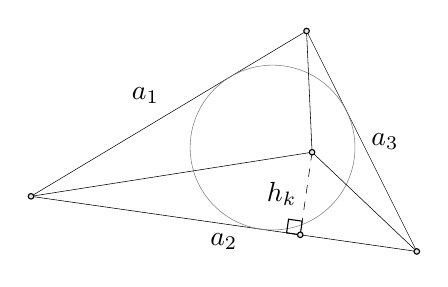
\begin{tikzpicture}[scale=0.7]
                \tkzDefPoint(0,1){A}
                \tkzDefPoint(7,0){B}
                \tkzDefPoint(5,4){C}
                \tkzDrawPolygon(A,B,C)

                \tkzDefCircle[in](A,B,C)
                \tkzGetPoint{O}
                \tkzGetLength{rIN}
                \tkzDefCircle[R](O, \rIN)
                \tkzGetPoint{a}
                \tkzDrawCircle(O, a)

                \tkzDefPoint(5.1, 1.8){P}
                \tkzDrawSegments(P,A P,B P,C)

                \tkzDefPointBy[projection=onto A--B](P)
                \tkzGetPoint{H}
                \tkzDrawSegment[dashed](P,H)

                \tkzLabelSegment[above left](A,C){$a_1$}
                \tkzLabelSegment[below](A,B){$a_2$}
                \tkzLabelSegment[right](B,C){$a_3$}

                \tkzMarkRightAngle(P,H,A)
                \tkzDrawPoints(A, B, C, P, H)
                \tkzLabelSegment[left](P,H){$h_k$}
            \end{tikzpicture}
        }
        \qquad
        \subfloat{
            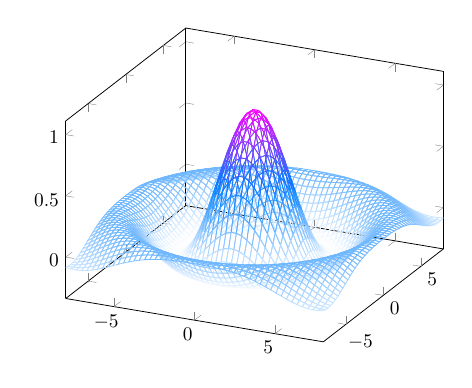
\begin{tikzpicture}[scale=0.7]
                \begin{axis}[
                        colormap/cool,
                    ]
                    \addplot3[
                        mesh,
                        samples=50,
                        domain=-8:8,
                    ]
                    {sin(deg(sqrt(x^2+y^2)))/sqrt(x^2+y^2)};
                \end{axis}
            \end{tikzpicture}
        }
    \end{figure}
\end{frame}

\begin{frame}
    \frametitle{\tex{}으로 무엇을 할 수 있나요?}

    다이어그램...

    \begin{figure}
        \centering
        \begin{circuitikz}
            \draw (0,0) node[ground, rotate=270]{} to [sV, v<=$v_{in}$]++(2,0) to [R=$R_E$]++(2,0) coordinate(Re) to [cI, l=$g_mv_\pi$, invert]++(3,0) coordinate(Rc) to [R=$R_C$]++(2,0) node[ground, rotate=90]{};
            \draw (Re) to [R, v<=$v_\pi$, l=$r_\pi$]++(0, -2) to [R=$R_B$]++(0,-2) node[ground]{};
            \draw (Rc) to [short, -o]++(0,-2) node[below]{$v_{out}$};
        \end{circuitikz}

    \end{figure}
\end{frame}

\begin{frame}[fragile]
    \frametitle{\tex{}으로 무엇을 할 수 있나요?}

    Syntax Highlighting...

    \begin{minted}{go}
        package main

        import "fmt"

        func main() {
            fmt.Println("Hello, World!")
        }
    \end{minted}

\end{frame}

\begin{frame}[fragile]
    \frametitle{\latex{} 문서의 구성}

    따라서 한 번 쳐보자.

    \begin{minted}{latex}
        \documentclass{oblivoir}
        \usepackage{kotex}

        \title{My First Document}
        \author{[당신의 이름]}

        \begin{document}
            \maketitle
            Hello, World! 안녕, 세계! $a^2 + b^2 = c^2$
            \[ E = mc^2 \]
        \end{document}
    \end{minted}

\end{frame}

\begin{frame}
\frametitle{preamble}

\mintinline{latex}{\begin{document}} 이전까지의 부분은 \textbf{preamble}이라고 부른다.preamble에는 보통 다음의 명령어들이 온다.

\begin{itemize}
    \item \mintinline{latex}{\documentclass}: 이 문서의 클래스를 결정한다. 클래스에 따라서 문서의 모양과 형식이 달라진다. 유명한 클래스로는 article, book, beamer, 그리고 앞으로 사용할 oblivoir 등이 있다.
    \item \mintinline{latex}{\usepackage}: 사용할 패키지들을 임포트한다. 텍에서의 패키지는 다른 언어의 패키지들과 유사하다.
    \item 기타 매크로 및 설정 (자세한 것은 3강에서 다룬다.)
\end{itemize}

\end{frame}

\begin{frame}[fragile]
    \frametitle{\latex{} 글 쓰기}

    \latex{}에서는 이어지는 화이트스페이스를 전부 하나의 빈 칸으로 대체한다.

    문단을 나눌 때는 반드시 한 줄을 비워놓는다. 화이트스페이스와 마찬가지로, 여러 줄을 비워놓아도 한 줄을 비운 것으로 인식한다.

    \begin{columns}[c]
        \column{0.4\textwidth}
        \begin{minted}[autogobble, showspaces]{latex}
            So,  so you think
            you can   tell

            Heaven  from hell?


            Blue skies from  pain?
        \end{minted}

        \column{0.4\textwidth}
        So,  so you think
        you can   tell

        Heaven  from hell?


        Blue skies from  pain?
    \end{columns}

\end{frame}

\begin{frame}[fragile]
    \frametitle{\latex{} 글 쓰기}

    다음의 문자들은 특수한 용도가 있으므로 일반적으로 입력할 수 없다.

    \begin{minted}{text}
        # $ % ^ & _ { } ~ \
    \end{minted}

    입력하고 싶다면, 앞에 \mintinline{text}{\}를 붙이면 된다. (\mintinline{text}{\#, \$, ...})

    \textbackslash는 \mintinline{text}{\textbackslash}로 입력한다.

\end{frame}

\begin{frame}[fragile]
    \frametitle{\latex{} 글 쓰기}

    따옴표는 왼쪽 따옴표와 오른쪽 따옴표가 구분된다. 왼쪽은 \mintinline{text}{`}, 오른쪽은 \mintinline{text}{'}이다. 비교해보자.

    \begin{center}
        \begin{tblr}{cc}
            \mintinline{text}{'Hello, World!'}   & 'Hello, World!'   \\ \hline
            \mintinline{text}{`Hello, World!'}   & `Hello, World!'   \\ \hline
            \mintinline{text}{``Hello, World!''} & ``Hello, World!'' \\
        \end{tblr}
    \end{center}

\end{frame}

\begin{frame}[fragile]
    \frametitle{\latex{} 글 쓰기}

    문서 구조는 크게 다음처럼 나눌 수 있다.

    \begin{itemize}
        \item part
        \item chapter
        \item section
        \item subsection
        \item paragraph
        \item subparagraph
    \end{itemize}

    보통 chapter, section, paragraph 정도만 본다.

\end{frame}

\begin{frame}[fragile]
    \frametitle{\latex{}의 명령어}

    \latex{}은 프로그래밍 언어이므로, 명령어의 개념이 있다. \latex{}의 명령어는 command와 environment로 분류할 수 있다.

    command는 다음과 같은 형식을 가진다.

    \begin{minted}{latex}
        \command[option1, option2, ...]{arg1}{arg2}...
    \end{minted}

    argument가 한 글자일 경우, 대괄호를 생략할 수 있다. 이 경우 토큰을 하나만 먹는다.

    \begin{center}
        \begin{tblr}{ll}
            \mintinline{latex}{\sqrt{2}} & $\sqrt{2}$ \\ \hline
            \mintinline{latex}{\sqrt 2 } & $\sqrt 2$  \\ \hline
            \mintinline{latex}{\sqrt 23} & $\sqrt 23$
        \end{tblr}
    \end{center}

\end{frame}

\begin{frame}[fragile]
    \frametitle{\latex{}의 명령어}

    environment는 다음과 같은 형식을 가진다.

    \begin{minted}{latex}
        \begin{environment}
            ...
        \end{environment}
    \end{minted}

    environment는 \mintinline{latex}{\begin}과 \mintinline{latex}{\end}로 둘러쌓인 구간에서 작동한다.

\end{frame}

\begin{frame}[fragile]
    \frametitle{\latex{}의 명령어}

    다음을 쳐 보자.

    \begin{minted}{latex}
        \begin{center}
            \textbf{Centered Text}: $\sqrt{2}$, $\sqrt[3]{2}$
        \end{center}
    \end{minted}

\end{frame}

\begin{frame}[fragile]
    \frametitle{유용한 명령어}

    다음과 같이 텍스트에 효과를 넣을 수 있다.

    \begin{center}
        \begin{tblr}{ll}
            \mintinline{latex}{\textbf{text}} & \textbf{text} \\ \hline
            \mintinline{latex}{\textit{text}} & \textit{text} \\ \hline
            \mintinline{latex}{\textsl{text}} & \textsl{text} \\ \hline
            \mintinline{latex}{\texttt{text}} & \texttt{text} \\
        \end{tblr}
    \end{center}

\end{frame}

\begin{frame}[fragile]
    \frametitle{유용한 명령어}

    다음과 같이 텍스트의 크기를 바꿀 수 있다.
    \begin{center}
        \begin{tblr}{ll}
            \mintinline{latex}{\tiny text}       & \tiny text       \\ \hline
            \mintinline{latex}{\small text}      & \small text      \\ \hline
            \mintinline{latex}{\normalsize text} & \normalsize text \\ \hline
            \mintinline{latex}{\Large text}      & \Large text      \\ \hline
            \mintinline{latex}{\Huge text}       & \Huge text       \\
        \end{tblr}
    \end{center}
    \textbf{이 효과는 문서 전체에 적용된다.} 이것이 싫다면 다시 \mintinline{latex}{\normalsize} 명령어를 사용하거나, 대괄호로 묶거나, 아니면 enviornment 형태로 사용하자.

\end{frame}

\begin{frame}[fragile]
    \frametitle{유용한 명령어}

    정렬을 변경하려면, \mintinline{latex}{flushleft, flushright, center} 환경을 사용한다.


    \begin{columns}[c]
        \column{0.4\textwidth}
        \begin{minted}[autogobble]{latex}
            \begin{flushleft}
                left aligned
            \end{flushleft}
            \begin{center}
                center aligned
            \end{center}
            \begin{flushright}
                right aligned
            \end{flushright}
        \end{minted}

        \column{0.4\textwidth}
        \begin{flushleft}
            left aligned
        \end{flushleft}
        \begin{center}
            center aligned
        \end{center}
        \begin{flushright}
            right aligned
        \end{flushright}
    \end{columns}

\end{frame}

\begin{frame}[fragile]
    \frametitle{유용한 명령어}

    글을 나열하는 방법으로는 \mintinline{text}{itemize, enumerate, description} 환경이 있다.

    \begin{columns}
        \column{0.3\textwidth}
        \begin{minted}[autogobble]{latex}
            \begin{itemize}
                \item a
                \item b
            \end{itemize}
        \end{minted}

        \begin{itemize}
            \item a
            \item b
        \end{itemize}

        \column{0.3\textwidth}
        \begin{minted}[autogobble]{latex}
            \begin{enumerate}
                \item a
                \item b
            \end{enumerate}
        \end{minted}

        \begin{enumerate}
            \item a
            \item b
        \end{enumerate}

        \column{0.3\textwidth}
        \begin{minted}[autogobble]{latex}
            \begin{description}
                \item[k1] a
                \item[k2] b
            \end{description}
        \end{minted}

        \begin{description}
            \item[k1] a
            \item[k2] b
        \end{description}
    \end{columns}

\end{frame}

\begin{frame}[fragile]
    \frametitle{폰트 바꾸기}

    폰트를 바꾸려면 \mintinline{text}{fontspec} 패키지를 로드한다. 이 패키지는 XeTeX과 LuaTeX에서만 사용할 수 있다.

    \begin{minted}{latex}
        \usepackage{fontspec}
        \setmainfont{serif font}
        \setsansfont{sans-serif font}
        \setmonofont{mono font}
    \end{minted}

    oblivoir 클래스 혹은 koTeX을 사용 중이라면, 다음 명령어를 이용해 한글 폰트를 바꿀 수 있다.

    \begin{minted}{latex}
        \setmainhangulfont{serif font}
        \setsanshangulfont{sans-serif font}
        \setmonohangulfont{mono font}
    \end{minted}

\end{frame}

\begin{frame}[fragile]
    \frametitle{용지 설정}

    oblivoir 클래스의 경우, \mintinline{text}{fapapersize} 패키지를 이용한다.

    \begin{minted}{latex}
        \usepackage{fapapersize}
        \usefapapersize{*,*,30mm,30mm,30mm,30mm}
    \end{minted}

    기타 클래스의 경우, \mintinline{text}{geometry} 패키지를 이용한다.
\end{frame}

\begin{frame}[c]

    \begin{center}
        백문이 불여일견, 직접 문서를 작성해보자!
    \end{center}

\end{frame}

\begin{frame}
    \frametitle{끝으로}

    \tex의 세계는 방대하기 때문에, 모든 것을 다 외운다는 생각은 버려야 한다.

    아래의 자료들과 구글을 활용해서, 그때그때 문제를 해결하면서 작성하도록 하자.

    \begin{itemize}
        \item lshort-ko -- 역사와 전통의 \latex 입문서이다.
        \item 권현우 교수님의 강의 -- 유튜브에서 무료로 볼 수 있다.
    \end{itemize}

\end{frame}

\begin{frame}[c]

    \begin{center}
        {\Huge Thank you for listening!}
    \end{center}

\end{frame}

\end{document}
